\chapter{The Description of a Set of Trajectories and Its Median Trajectory}
\label{chap:definition}

\section{Set of Trajectories}
\label{sec:setoftrjs}

In this thesis, we only consider the spatial component of the trajectory. 
Therefore, we represent a trajectory as a polygonal line built by a series of points and connected by line segments.   
 
Let $T:=\{\tau_{1},\tau_{2},...,\tau_{m}\}$ be the input set of $m$ trajectories for which we want to compute its median trajectory $\tau^{M}$.
We define each trajectory in $T$ as a list of at most $n$ points, $\tau_{i}:=(p_{i,1},...,p_{i,k})$ where $1 \leq i \leq m$ and $2 \leq k \leq n$. 
Note that the number of points for each trajectory can be different.
Every two consecutive points $p_{i,j}$ and $p_{i,j+1}$ $(1 \leq j \leq k-1)$ are connected by a segment $s_{i,j}:=(\overline{p_{i,j},p_{i,j+1}})$.

$P$ is the set of all points in $T$, $P:=\{p_{i,j} \mid i \in \{ 1 ... m\} , j \in \{ 1 ... n\} \}$ and $S$ is the set of all segments in $T$, $S:=\{s_{i,j} \mid i \in \{ 1 ... m\} , j \in \{ 1 ... n-1\} \}$.
All trajectories in $T$ share the same start and end points $(p_{1,1}=p_{2,1}=...=p_{m,1}$ and $p_{1,k_{1}}=p_{2,k_{2}}=...=p_{m,k_{m}}$ where $ \{k_{1},...,k_{m}\} \in \{1,...,n\})$. 

Trajectories can intersect with other trajectories in other points than their start and end points.
These intersection points are also included in the list of points that define the trajectory. When two segments intersect each other, then both segments will be split into two parts and all four segments share one intersection point as one of their endpoints (see Figure~\ref{fig:number_trj}).

\begin{figure}
\centering
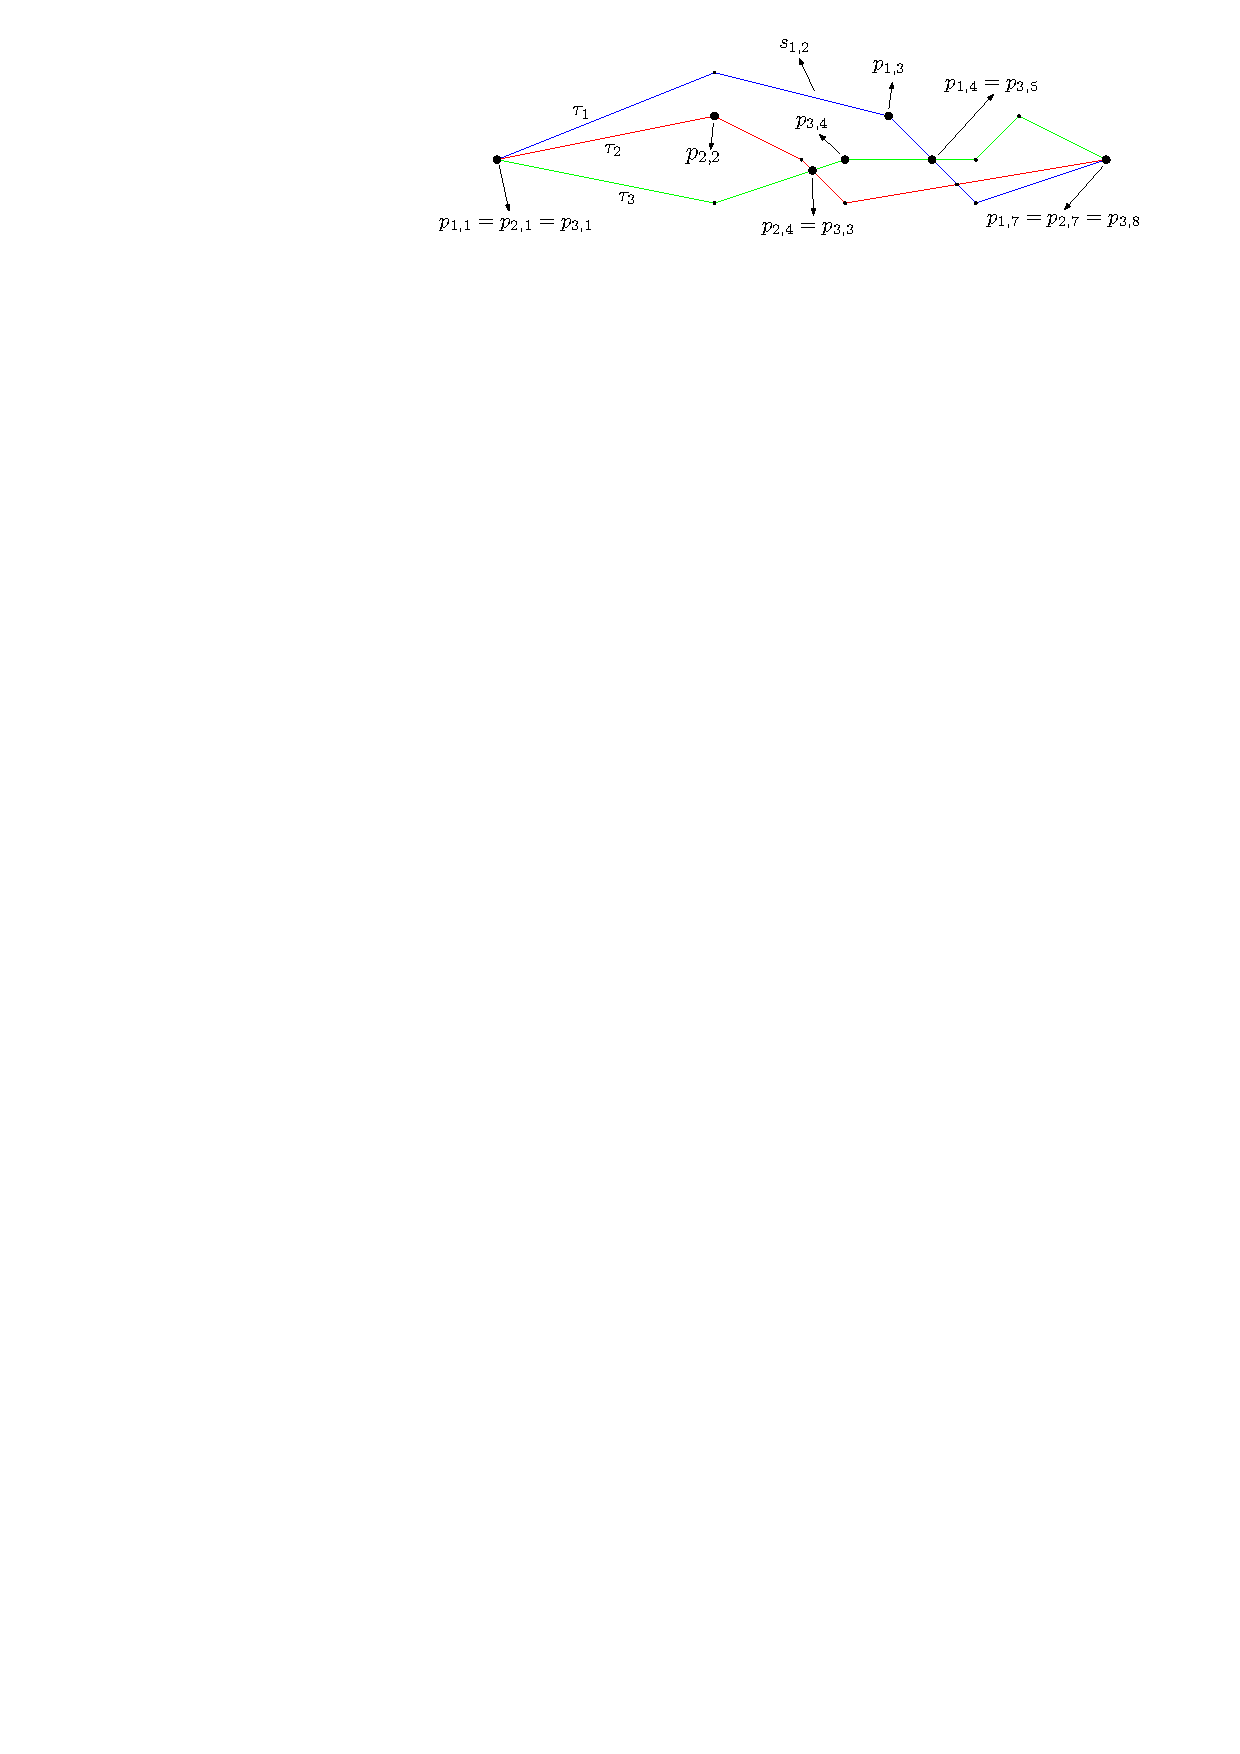
\includegraphics[scale=0.8]{Gambar/number_trj}
\caption[Numbering of points and segments]{Numbering of points and segments} 
\label{fig:number_trj}
\end{figure}

Let $n'$ be the number of points in a trajectory, including their intersection points with other trajectories. 
In the worst case, $n' = mn^{2}$. 
In the rest of this thesis, we define $n$ as a number of points in a trajectory, inclusive with its intersection points with other trajectories. 
Note that the number of segments for each trajectory is linear to the number of points, because trajectory with $n$ points has $n-1$ segments.

\section{Properties of the Median Trajectory}
\label{sec:prop_medtrj}

We define several properties for the median trajectory  $\tau^{M}$ with respect to the input set of trajectories $T$:

\begin{itemize}
\item 
$\tau^{M}$ is a directed polygonal line from start point to end point and should be similar to most trajectories in $T$.

\item 
It must be built only using points and segments which are parts of trajectories in the input set. 

\item 
The usage of segments should follow the direction of them. Therefore, it is not allowed to use a segment such that the direction of $\tau^{M}$ is opposite to the direction of that segment in a trajectory (see Figure~\ref{fig:forbid_seg}, indicated by the dark blue arrow).

\begin{figure}
\centering
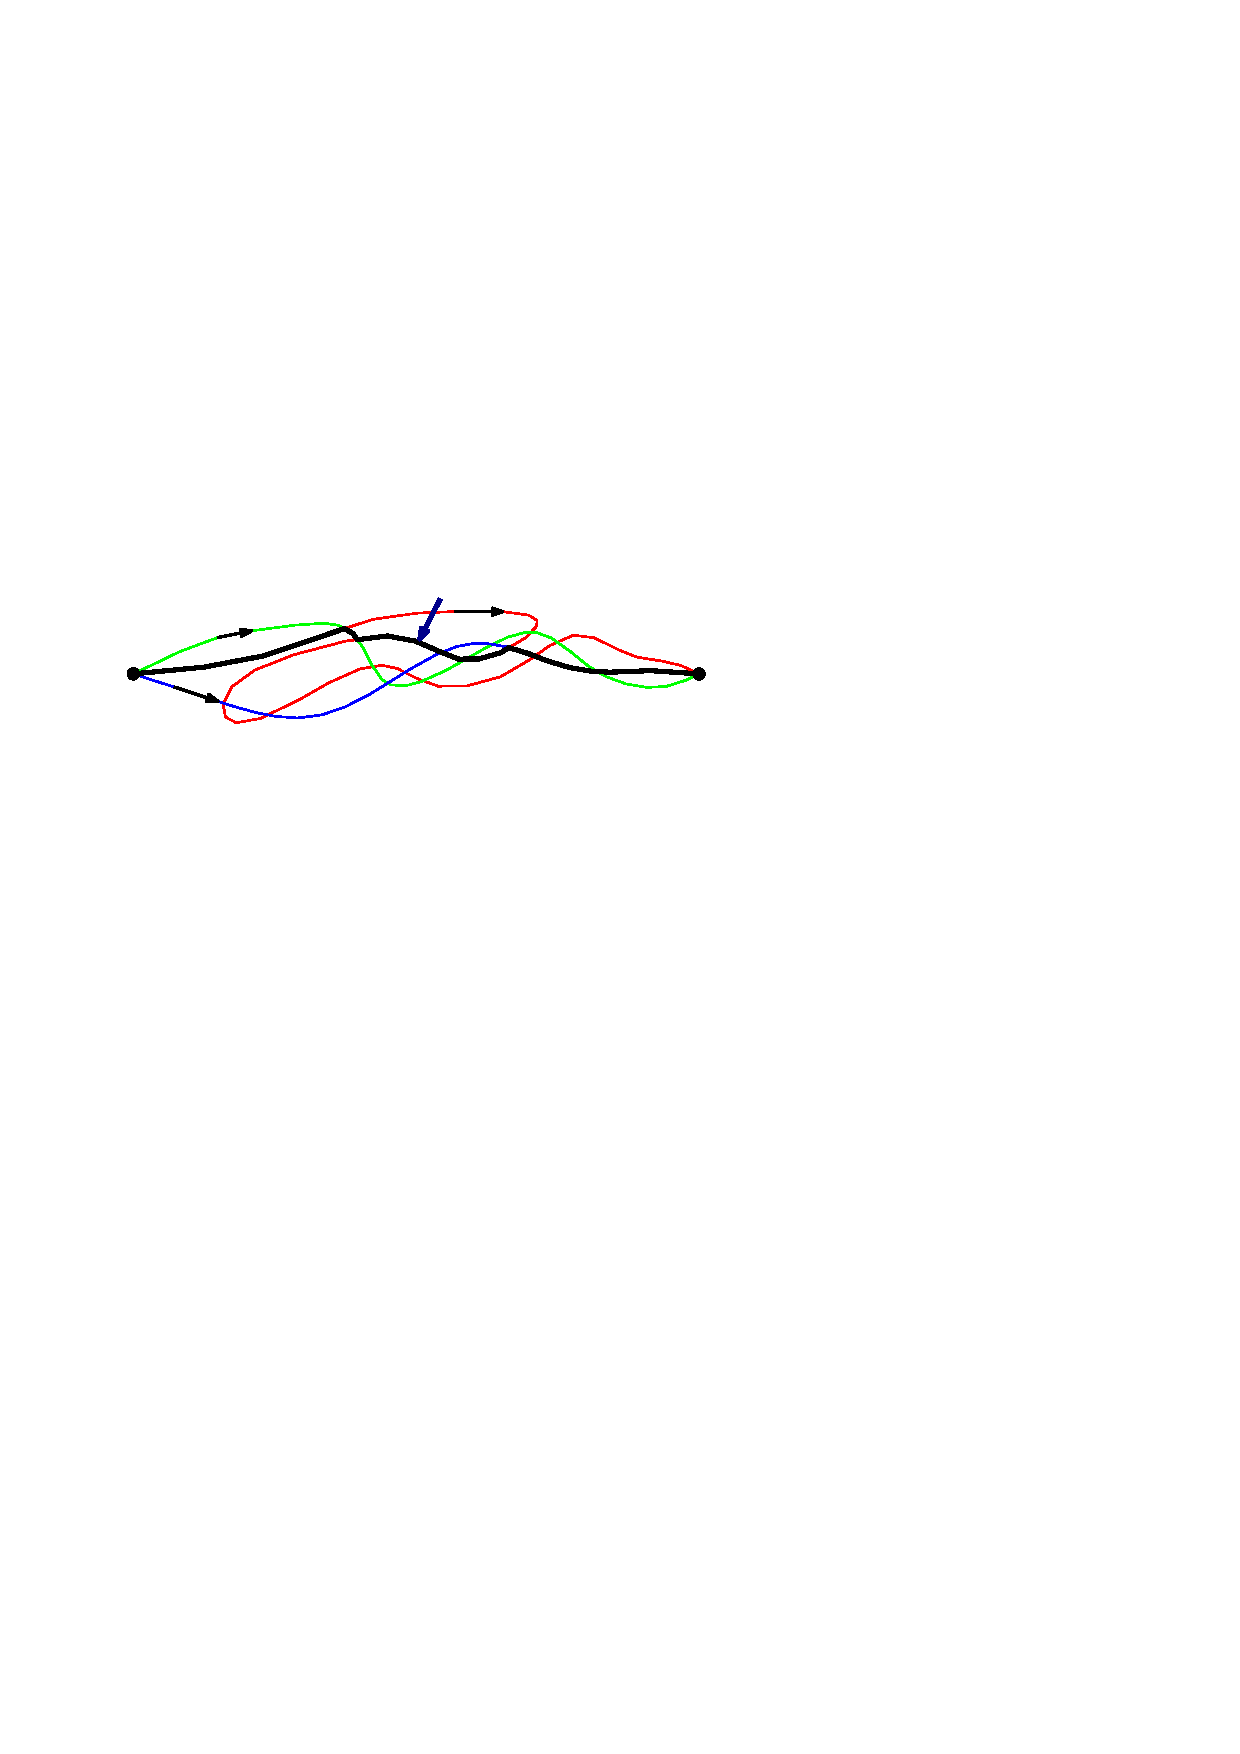
\includegraphics[scale=0.9]{Gambar/forbid_seg}
\caption[Possible median trajectory (in black) with backward direction (pointed by the blue arrow)]{Possible median trajectory (in black) with backward direction (indicated by the blue arrow)} 
\label{fig:forbid_seg}
\end{figure}

\item 
The length of the median trajectory should be relatively the same as the average length of all trajectories in the input set.

\item 
The total angular change should also be similar to the average of total angular change of all trajectories in the input set.
The total angular change of a trajectory is the sum of all angular changes at every vertex in that trajectory (see Figure~\ref{fig:total_ang}). 

\begin{figure}
\centering
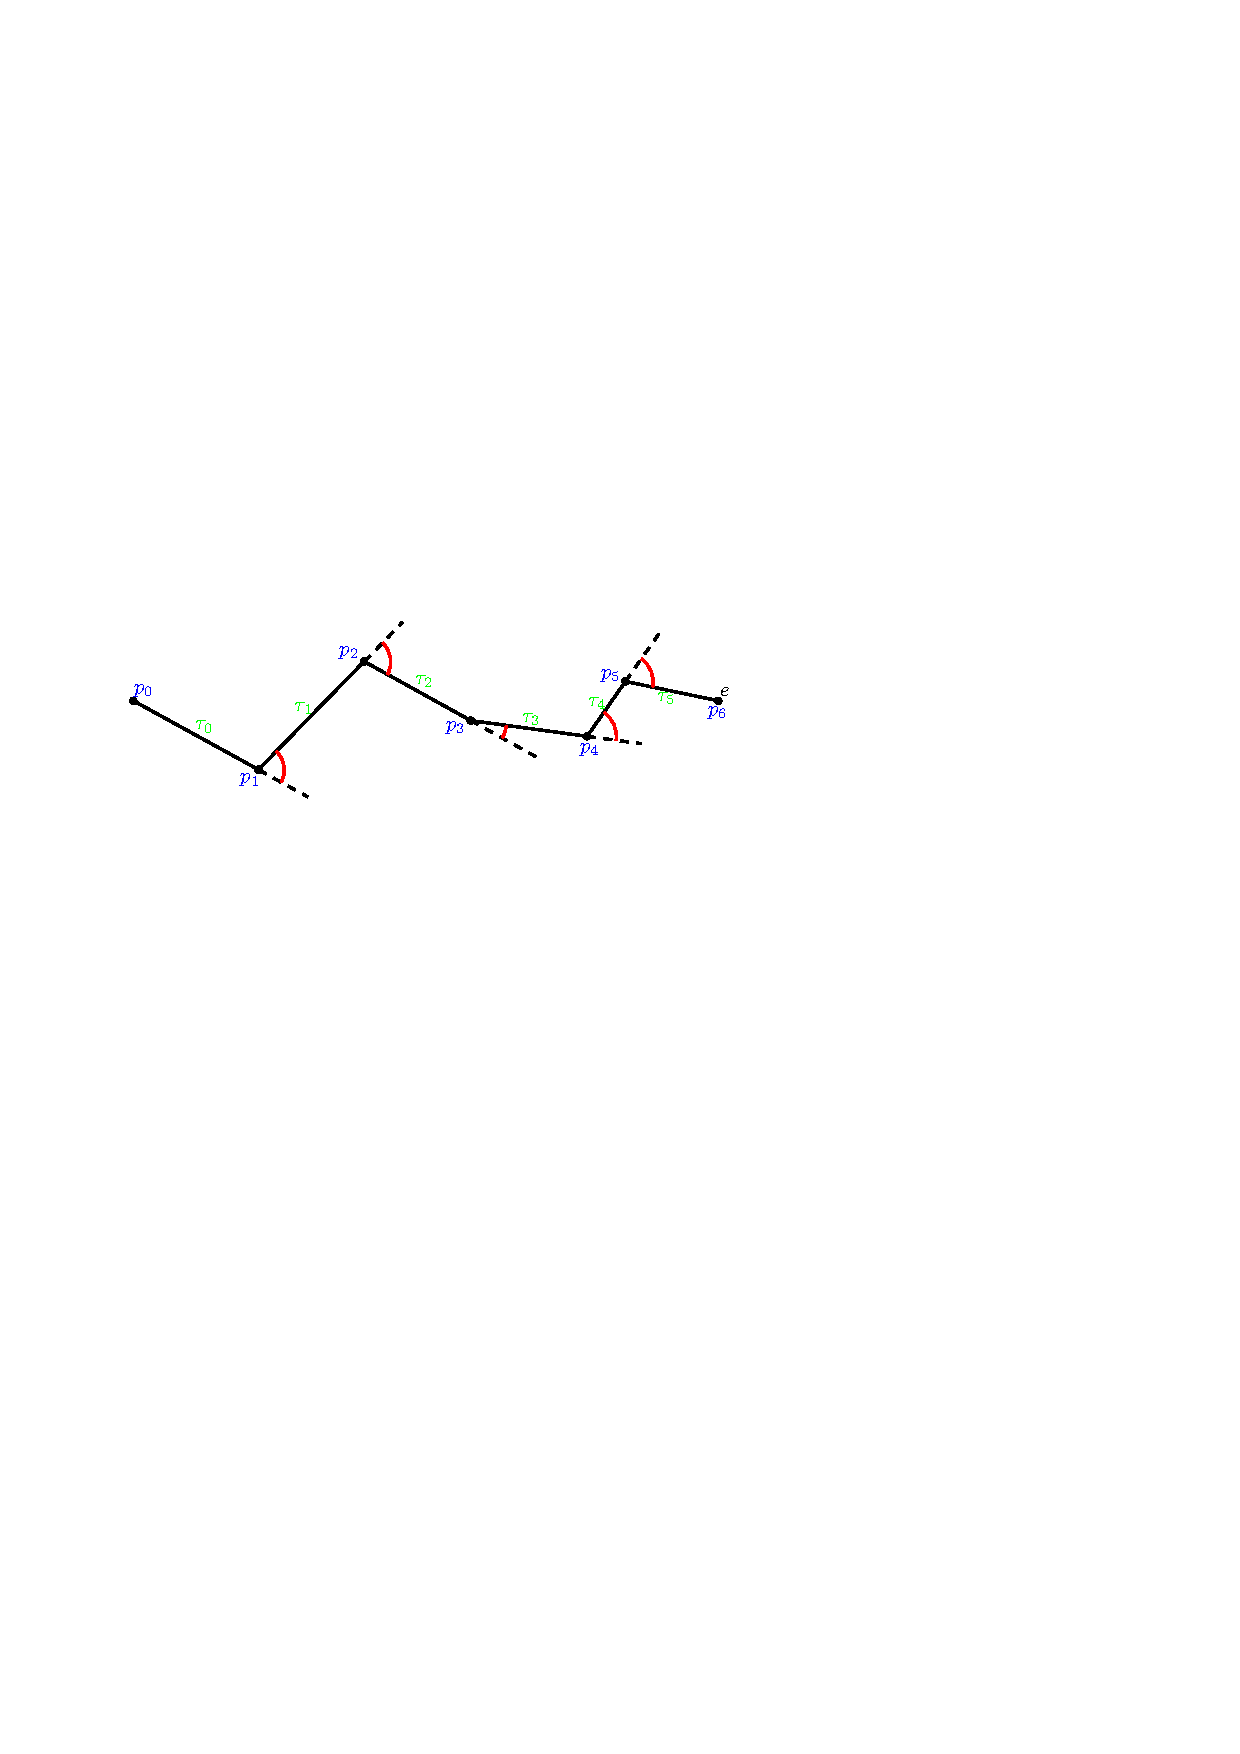
\includegraphics[scale=1]{Gambar/total_ang}
\caption[Red arcs indicate the angular change at each vertex]{Red arcs indicate the angular change at each vertex} 
\label{fig:total_ang}
\end{figure}

\item 
The number of vertices and edges of $\tau^{M}$ should be about the same with the average of the number of vertices and edges from all trajectories in the input set.
		%\item The final result of $\tau^{M}$ should not be influenced by an outliers.  
\end{itemize}


Using the definition of the input set of trajectories defined in the previous section, we define a median trajectory $\tau^{M}$ as a sequence of points from $T$, $\tau^{M}:=(p_{i_{1},j_{1}},p_{i_{2},j_{2}},...,$ $p_{i_{k},j_{k}})$ where $\{i_{1},i_{2},...,i_{k}\} \in \{1 ... m\}$ and $\{j_{1},j_{2},...,j_{k}\} \in \{ 1 ... n\}$, or defined as a sequence of segments: $\tau^{M}:=(s_{i_{1},j_{1}},s_{i_{2},j_{2}}, ...,s_{i_{k},j_{k}})$ where $\{i_{1},i_{2},...,i_{k}\} \in \{1 ... m\}$ and $\{j_{1},j_{2},...,j_{k}\} \in \{1 ... n-1\}$. 
Note that $\tau^{M}$ and all trajectories in $T$ share the same start point and end point.   


%  

Table~\ref{tab:tab_begin} shows how this information is kept in $\Gamma$. 
\begin{table}
\centering
\caption{Table $\Gamma$ after inserting $\mathcal{S}_{1}$}
\label{tab:tab_begin}
\begin{tabular}{cccc}
\toprule

 & $v_{start}$ & $\mathcal{S}_{1}$ & $v_{end}$\\
\midrule
$\tau_{1}$ & 1 & 12& 20\\
$\tau_{2}$ & 1 &  & 20\\
$\tau_{3}$ & 1 & 9 & 20\\
$\tau_{4}$ & 1 &  & 20\\
\bottomrule
\end{tabular}
\end{table}

There are two possibilities of the placement of $\mathcal{S}_{2}$: 
\begin{table}[H]
\begin{minipage}[c]{0.49\linewidth}
\centering
\caption{$\mathcal{S}_{2}$ between $v_{start}$ and $\mathcal{S}_{1}$}
\label{tab:tab_next1}
\begin{tabular}{ccccc}
\toprule

 & $v_{start}$ & $\mathcal{S}_{2}$ & $\mathcal{S}_{1}$ & $v_{end}$\\
\midrule
$\tau_{1}$ & 1 & 5 \cellcolor{green}& 12& 20\\
$\tau_{2}$ & 1 & 8 \cellcolor{green}& & 20\\
$\tau_{3}$ & 1 & 2/8/17 \cellcolor{green}& 9 & 20\\
$\tau_{4}$ & 1 & \cellcolor{red}& & 20\\
\bottomrule
\end{tabular}
\end{minipage}
\begin{minipage}[c]{0.49\linewidth}

\centering
\caption{$\mathcal{S}_{2}$ between $\mathcal{S}_{1}$ and $v_{end}$}
\label{tab:tab_next2}
\begin{tabular}{ccccc}
\toprule

 & $v_{start}$ & $\mathcal{S}_{1}$ & $\mathcal{S}_{2}$ & $v_{end}$\\
\midrule
$\tau_{1}$ & 1 & 12& 5 \cellcolor{red} &20\\
$\tau_{2}$ & 1 &  &  8 \cellcolor{green} &20\\
$\tau_{3}$ & 1 & 9 & 2/8/17 \cellcolor{green} &20\\
$\tau_{4}$ & 1 &   & \cellcolor{red} &20\\
\bottomrule
\end{tabular}
\end{minipage}
\end{table}

The final placement of table $\Gamma$ after simplification: 
\begin{table}[H]
\centering
\caption{Final $\Gamma$}
\label{tab:tab_final}
\begin{tabular}{ccccc}
\toprule
 & $v_{start}$ & $\mathcal{S}_{2}$ & $\mathcal{S}_{1}$ & $v_{end}$\\
\midrule
$\tau_{1}$ & 1 & 5 & 12& 20\\
$\tau_{2}$ & 1 & 8 &   & 20\\
$\tau_{3}$ & 1 & 8 & 9 & 20\\
$\tau_{4}$ & 1 &   &   & 20\\
\bottomrule
\end{tabular}
\end{table}

